%----------------------------------------------------------------------------------------
%	PACKAGES AND OTHER DOCUMENT CONFIGURATIONS
%----------------------------------------------------------------------------------------
\documentclass[margin, centered]{res}
\topmargin=-.4in
\oddsidemargin -0.3in
\evensidemargin -.1in
\textwidth=4.5in
\itemsep=0in
\parsep=0in
\newsectionwidth{1in}
\usepackage[pdftex]{graphicx}
\usepackage{wrapfig}
\usepackage{helvet}
\usepackage[colorlinks = true,
            linkcolor = blue,
            urlcolor  = blue,
            citecolor = black,
            anchorcolor = black]{hyperref}
\setlength{\textwidth}{6in} % Text width of the document
\setlength{\textheight}{720pt}
\usepackage{enumitem}
\setlist[itemize]{topsep=2pt,itemsep=2pt,parsep=0pt,partopsep=0pt}
\begin{document}

%----------------------------------------------------------------------------------------
%	NAME AND ADDRESS SECTION
%----------------------------------------------------------------------------------------\
\setlength{\voffset}{0.1in}
\begin{center}
    
 %   \LARGE\bf{\href{https://www.hridaydutta123.github.io}{Hridoy Sankar Dutta}} \\
 %   \normalsize{hridoysankardutta@gmail.com, +447469674172}\\
 %   \normalsize{UK Permanent Resident (No Visa Sponsorship Required)}
    
%\smash{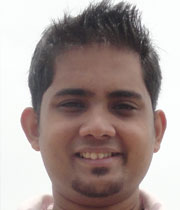
\includegraphics[width=2cm]{hridoyd.jpg}}
\end{center}
\vspace{-6mm}
\hfill
\vspace{-7mm}
\begin{resume}
\section{Professional Highlights}
\begin{itemize}[leftmargin=*]

\item Senior AI Researcher and Academician with 8+ years of experience working at the intersection of cybersecurity, data science, and large-scale online systems, focusing on measurement and analysis of complex digital ecosystems.

\item Extensive experience designing and managing large-scale datasets and automated data pipelines for scientific research, including the development of widely used open-source datasets. The datasets have received 1500+ downloads and have been adopted by industry (e.g., ActiveFence) and academia for cybercrime analysis,  social media intelligence and large-scale online safety research.

\item Proven ability to conduct interdisciplinary research and collaborate across domains, with academic experience at the University of Cambridge and Deakin University, translating complex technical insights to diverse research and engineering teams.

\item Published impactful research in leading peer-reviewed conferences and journals including TIFS, ASIACCS, WiSec, eCrime, TIST, ICWSM, CIKM, and WSDM, demonstrating strong experience in rigorous data-driven scientific research.

\end{itemize}
%----------------------------------------------------------------------------------------
%	WORK EXPERIENCE SECTION
%----------------------------------------------------------------------------------------
\section{Experience \& Education}
\textbf{Lecturer in Cybersecurity, Deakin University, Australia} \hfill July 2024 - Present\\ 
\emph{GIFT City Campus}\\
\textbf{Research Associate, University of Cambridge} \hfill June 2021 - June 2024\\
\emph{Cambridge Cybercrime Centre \\
University of Cambridge
} \\
\\ [-2mm]
\textbf{Research Assistant, University of Cambridge} \hfill February 2021 - June 2021\\
\emph{Cambridge Cybercrime Centre \\
University of Cambridge
} \\\\ [-2mm]
\textbf{PhD in Computer Science and Engineering} \hfill August 2017 - September 2021 \\
Indraprastha Institute of Information Technology Delhi (IIIT-D)



\section{Datasets}
\begin{itemize}[leftmargin=*]
\item GONets:  A first-look into GitHub Organisation Networks [SIGIR'26].
\item YT-30M: A multi-lingual multi-category dataset of YouTube comments [CIKM'25].\\
\textit{\small{HuggingFace downloads: 691}},
\textit{\small{Industry adoption: ActiveFence (Alice)}}
\item ABOME: A Multi-platform Data Repository of Artificially Boosted Online Media Entities. [ICWSM'21]\\
\textit{\small{Zenodo downloads: 711}}
\item ModZoo: A large-scale dataset of 159K modded Android apps through longitudinal measurement of 13 major modded app marketplaces. [eCrime'24]
\item iOSModZoo: Built large-scale datasets of 40K modded iOS apps and 77K App Store counterparts through 11-month monitoring of 9 modded markets, enriched with metadata from 1.02M official iOS apps. [WiSec'26]
\end{itemize}
\section{Open-source contributions}
\begin{itemize}[leftmargin=*]
\item The YouTube Scraper - Tool to download YouTube video descriptions and comments without using the YouTube API. \textit{(160+ stars, 25+ forks)}
\item Awesome Twitter Tools - A curated list of Twitter tools  and resources. \textit{(200+ stars, 25+ forks)}

\end{itemize}
\section{Interests and Skills}
\begin{itemize}[leftmargin=*]
 \item[] \textbf{Interests:} Data-driven cybersecurity, Cybercrime,  Social network safety, LLM Safety.
 \item[] \textbf{Operating systems}: GNU/Linux; \textbf{Tools}: Python, SQL, Deep Learning (Graphs), GitHub.
\end{itemize}

\section{Grants}
\textbf{Deakin University Peer-review ECR Support Scheme} \hfill 4250 AUD  \\
\textbf{Deakin University SIT Minor Equipment \& Expenses Scheme 2025} \hfill 3500 AUD  \\
\textbf{Deakin University Startup Grant (PI)} \hfill INR 10000 AUD  \\
\textbf{Deakin Cyber Collaboration Grants Scheme 2025 (Co-PI)} \hfill 5000 AUD  \\
\emph{Deakin University} 

\textbf{OpenAI Researcher Access Program (PI)} \hfill 1000 USD  \\
\textbf{Cohere Labs Catalyst Grant Program} \hfill 500 USD 

\section{Other Experiences}
\begin{itemize}[leftmargin=*]
\item[] \textbf{Co-founder,  Assam AI Initiative (AAII)} \\
\emph{A non-profit initiative to promote various scopes of AI} \hfill Feb 2021 - Present
\item[] \textbf{Visiting Researcher, TU Munich, Germany} \hfill July 2023
%\emph{Supervisor: Prof. Juergen Pfeffer\\ Professor of Computational Social Science \& Big Data, TU Munich}  \\
\item[] \textbf{Visiting Researcher, Cardiff University, UK} \hfill March 2019,  March 2020
%\emph{Supervisor: Prof. Pete Burnap \\ Professor, School of Computer Science and Informatics, Cardiff University} \hfill March 2019,  March 2020 \\
\item[] \textbf{Short-Term Scholar, George Mason University, USA} \hfill June 2019 - August 2019
\end{itemize}
%\emph{Supervisor: Dr. Hemant Purohit,  Associate Professor, Information Sciences \& Technology Department \\ George Mason University (GMU)}  \\

\section{Achievements and Awards}
\begin{itemize}[leftmargin=*]
 \item Rising Star in Data Science by the Center for Data and Computing (CDAC), University of Chicago.
 \item Wiseman Prize 2023, Department of Computer Science and Technology, University of Cambridge.
 \item DAAD AInet fellowship 2023.
 \item SEBE Teaching Award, Deakin University.
 \item ICWSM 2021 scholarship for Underrepresented Groups Program.
 \item 3rd prize at Ninth IDRBT Doctoral Colloquim IDC 2019.
\end{itemize}

\end{resume}
\end{document}